\section{Redundant file characterization}
\label{sec:redundant_files}

In this section, we present our redundant file characterization on file repeat count, file size, and file types. 
Based on this characterization, we create three-level classification hierarchy as shown in Figure~\ref{fig:class-hierarchy}.
At the highest level, we created two categories: \textit{common redundant file types and non-common redundant file types}. 
The majority (xxxx\% files, with xxx TB) are common file types that consists of a largest number of redundant files with large storage space consumed, such as xxx and xxx. 
Only xxxx\% files are non-common file types that only contains a small number of redundant files with less storage space, such as xxxx and xxxx. 
Since our focus is on the major redundant files, our further classification expands on the xxx\% common redundant file types.  

At the second level of the hierarchy, we clustered common redundant file types based on the \textit{major usage, platform, or framework} involved by each file type. We identified redundant files' types relevant to \textit{archival, productivity, programming languages, scripts, images, databases, executables, and others}.

At the third level, we classified the redundant files based on the specific file type or extension. Totally, we get around 690 types. 
%We selected the file types which take largest storage space.  

Based on the second-and third-level classification, we further investigated the following two research questions: (1) What are the common redundant files?
(2) Why there are so many redundant files? and present our investigation results.

\begin{figure}
	\centering
	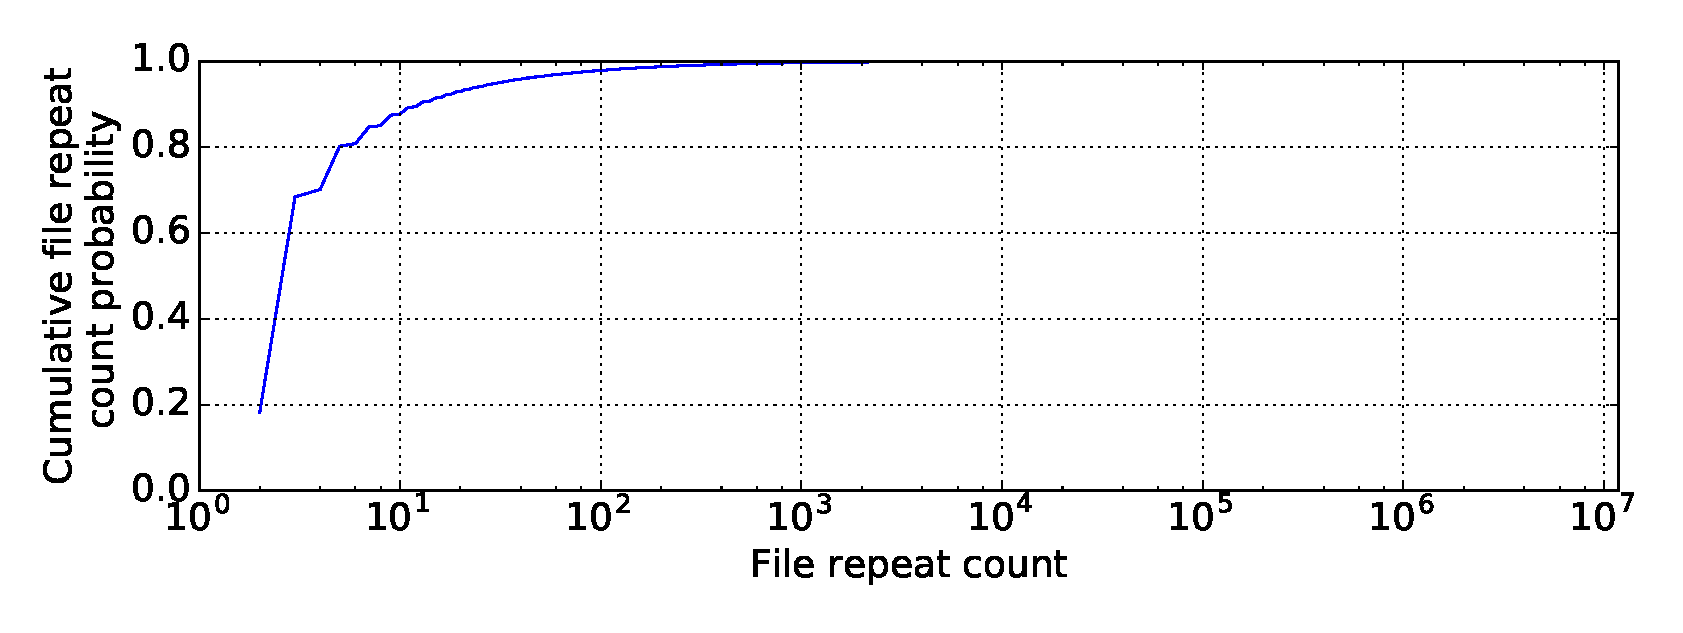
\includegraphics[width=0.5\textwidth]{graphs/File_repeat_count.eps}
	\caption{File repeat count distribution.
	}
	\label{fig:file-repeat-cnt}
\end{figure}

Figure~\ref{fig:file-repeat-cnt} shows the cumulative and probability distribution of file repeat count. 
Most files have a small repeat count. For instance, almost 90\% of files have equal or less than 10 copies. Around 50\% of files have 4 copies.
The file that has the maximum repeat count is empty file, which means that many users creates empty files and stored in their images.
%\subsection{File repeat count}
%\subsection{File size}

\begin{figure}
	\centering
	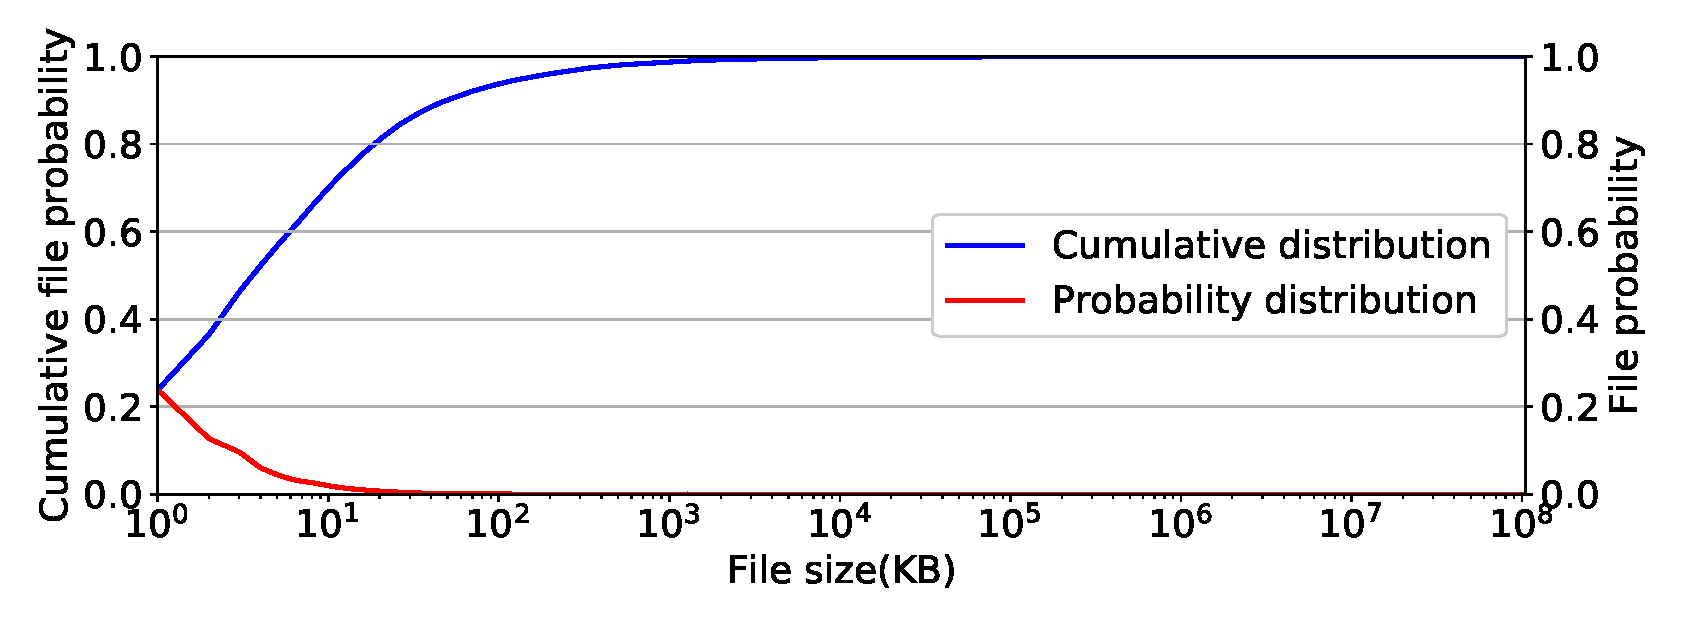
\includegraphics[width=0.5\textwidth]{graphs/File_size-KB.eps}
	\caption{File size distribution.
	}
	\label{fig:file-size}
\end{figure}

Figure~\ref{fig:file-size} shows the cumulative and probability distribution of file size of unique dataset after we remove the redundant files.
Most files are smaller files. For example, 91\% files'sizes are equal or less than 100KB. 
Around 22\% of files are less than 1 KB.
 

\subsection{Overview of common redundant file types}

\begin{figure}
	\centering
	\subfigure[Top redundant file types in terms of file count.]{\label{fig:dedup_cdf}
		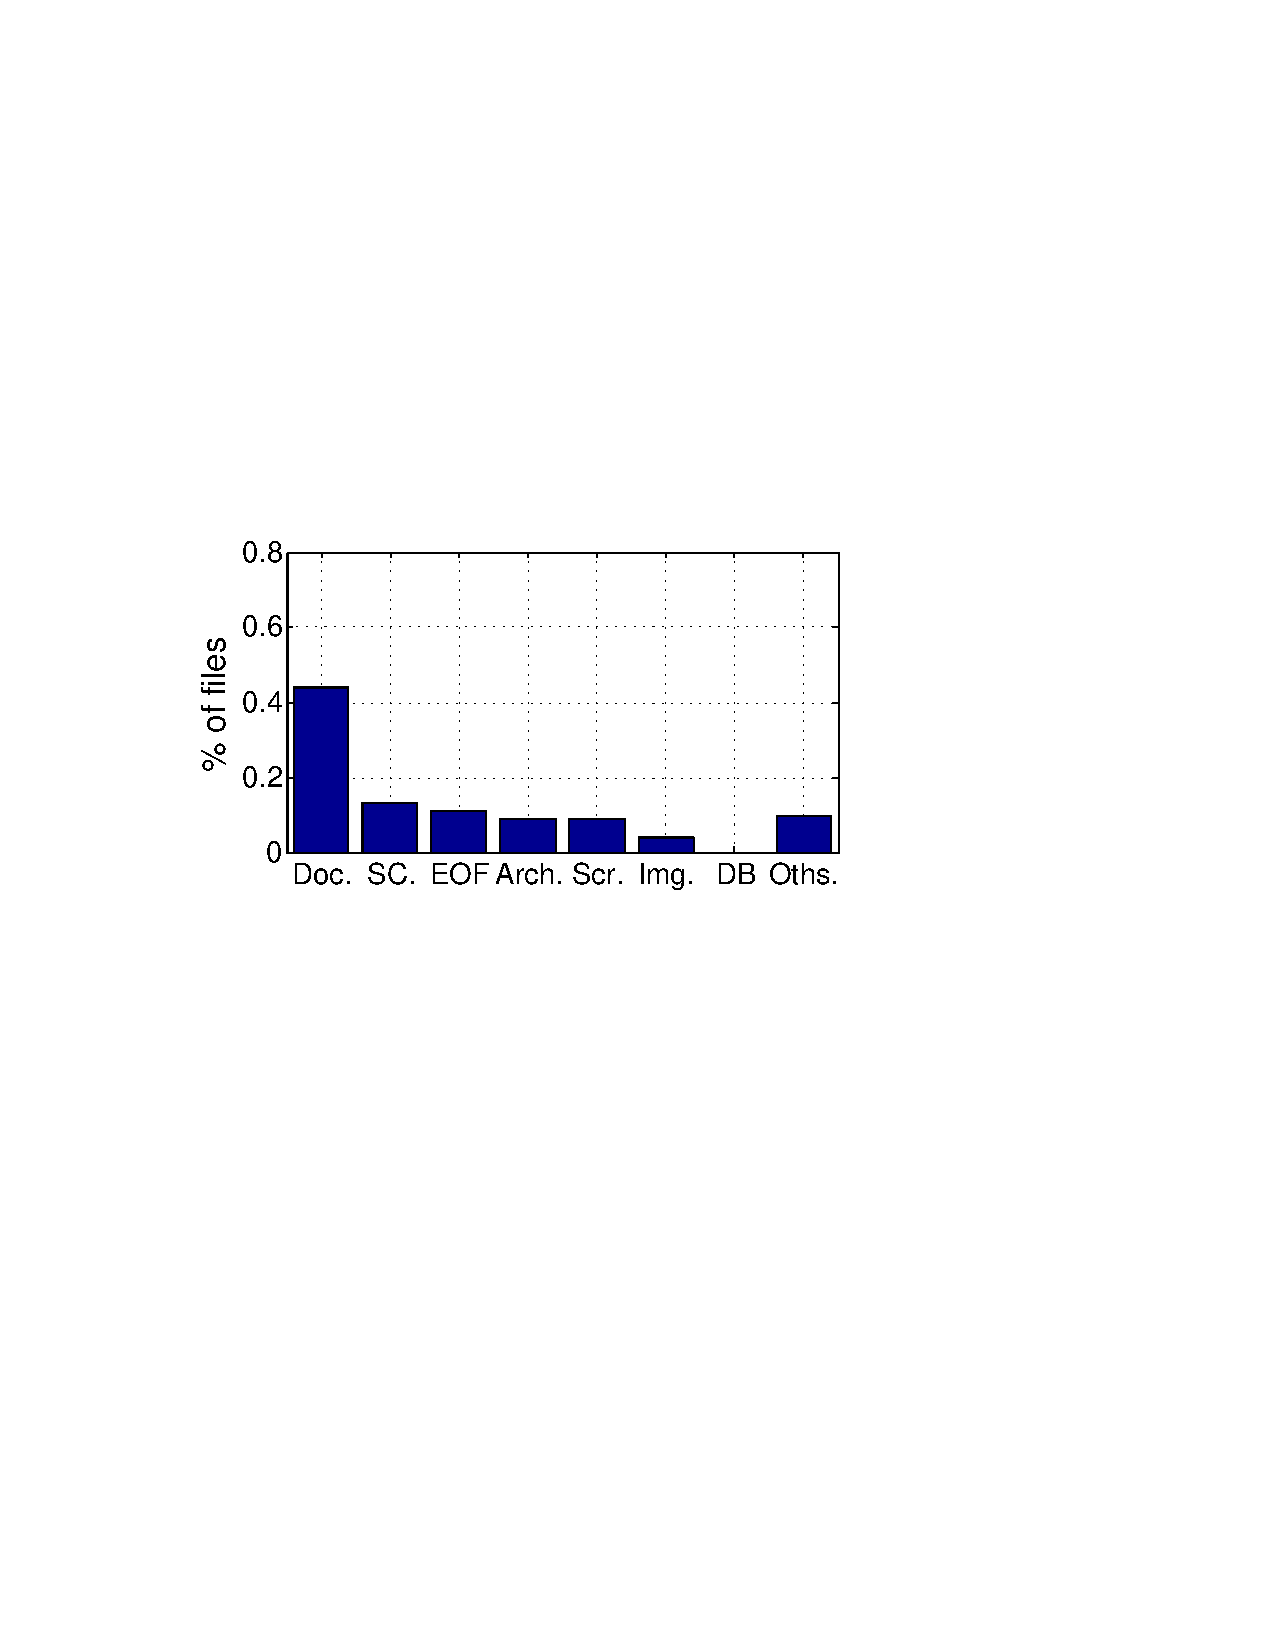
\includegraphics [width=0.4\textwidth]{graphs/type-total-cnt}
	}
	\subfigure[Top redundant file types in terms of capacity.]{\label{fig:dedup_hist}
		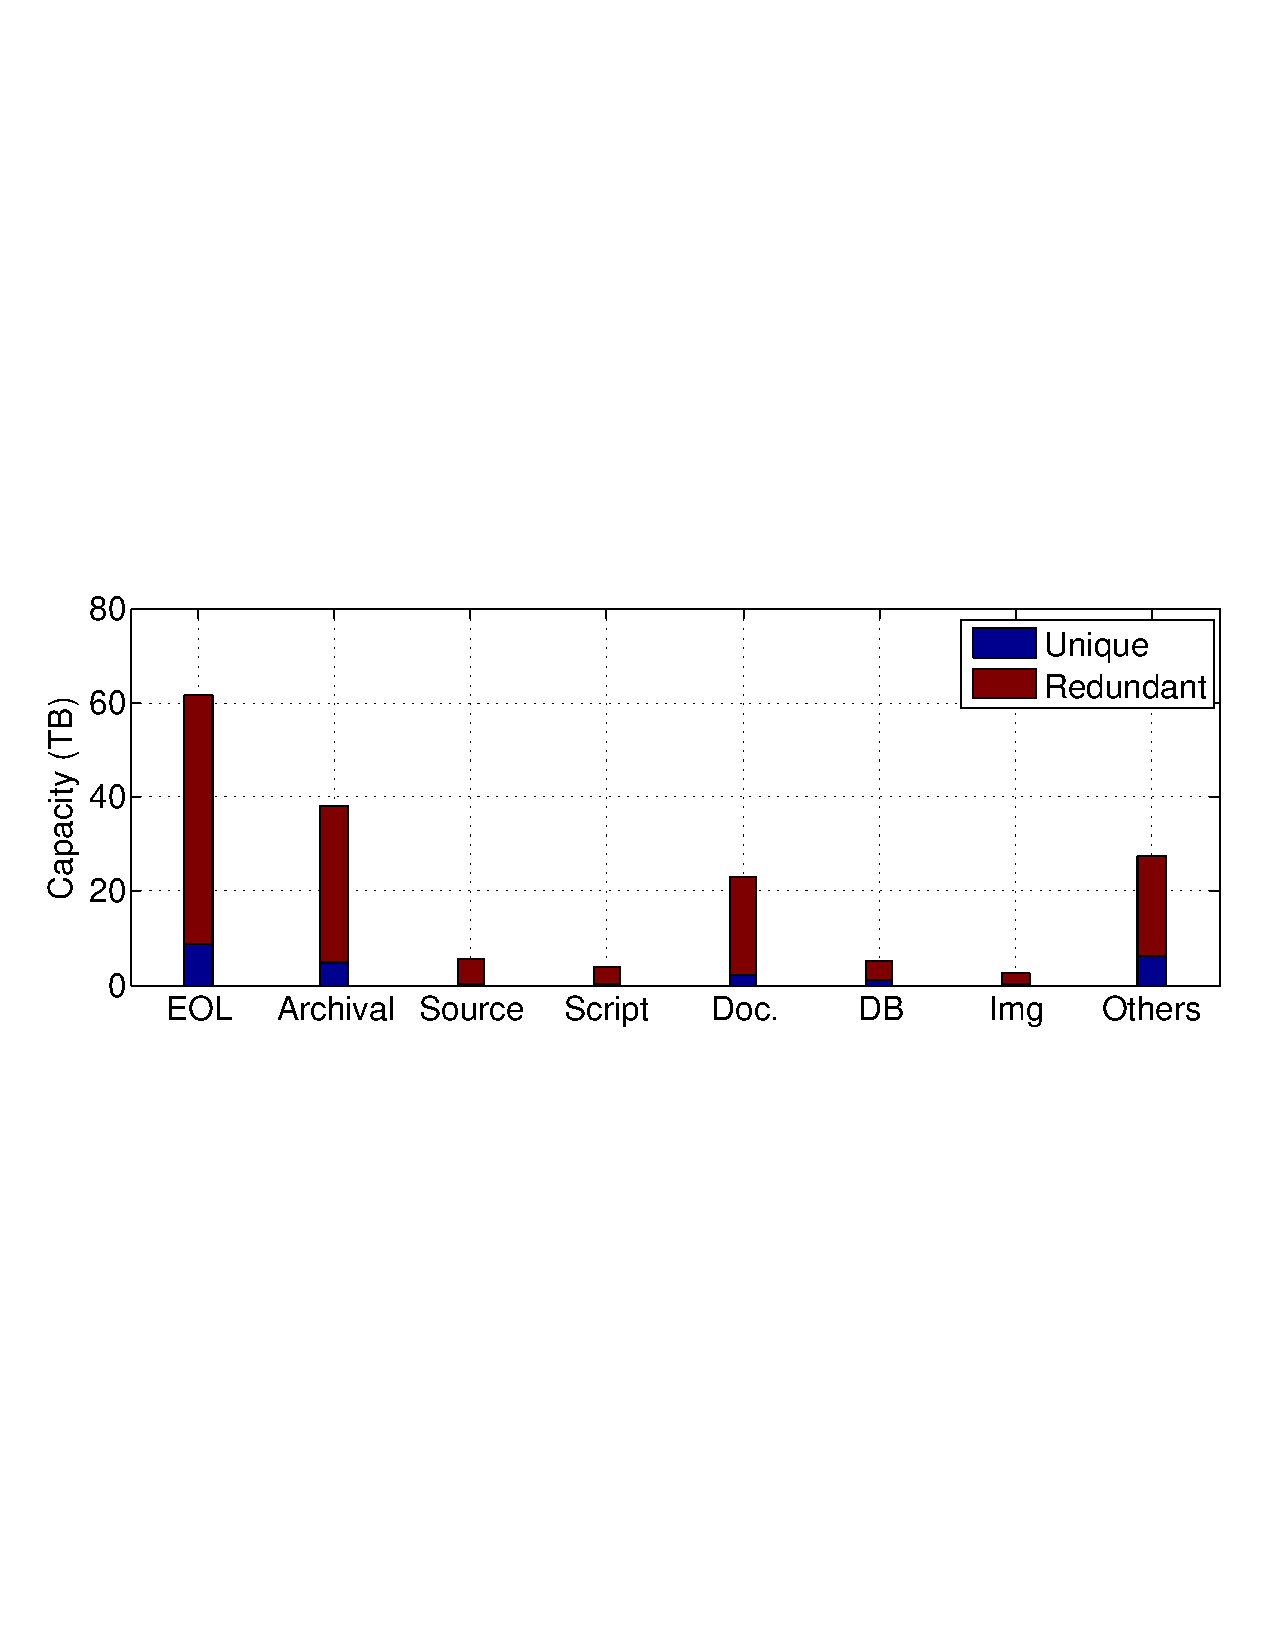
\includegraphics [width=0.4\textwidth]{graphs/type-total-cap}
	}
	\caption{Top redundant file types}
	\label{fig:file-types}
\end{figure}

\subsection{Executable}

A large executable group is ELF file type, which consists of ELF 64/32-bit LSB relocatable, shared object, executable, core file, processor-specific for x86-64, MIPS,
ARM, Intel 80386, etc. architectures.
Another executable group contains VAX COFF executable, PE32/PE32+ executable for Windows, and 386 pure executable, VMS Alpha, etc.
\% of files are script executable, which contains python, shell, etc.
\% of files are RPM, Debian bin
%The last group contains

Figure~\ref{fig-elf}
\subsection{Lib}

library files contains libtool library file, OCaml native library, MIT scheme, Mach-O library, OCaml library, Palm OS dynamic library data, Microsoft c/c++ library.current ar archive random library, and other library.
%libtool\|OCaml\|Palm\|MIT\|microsoft\|current ar archive random library\|mach-o\|rpm\|gzip

\subsection{Programming languages \&. scripts}

\begin{figure}
	\centering
	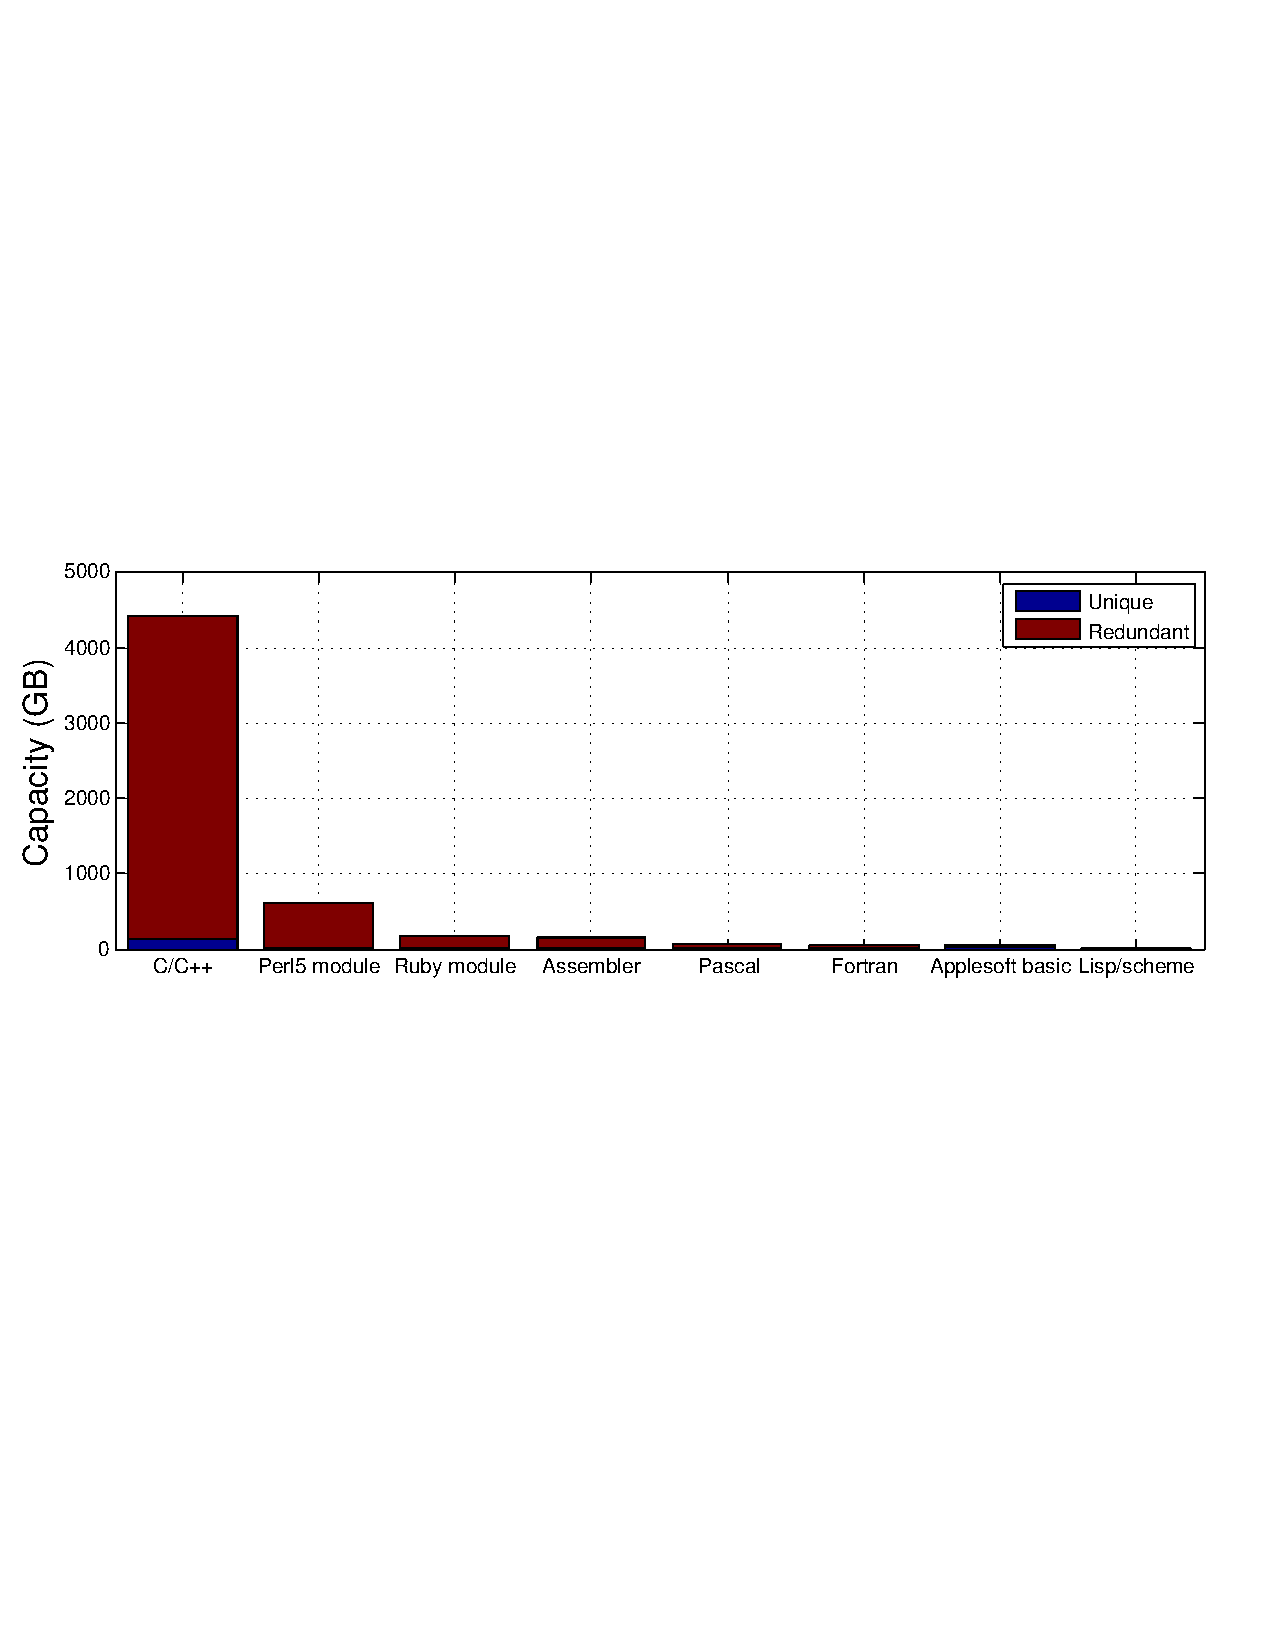
\includegraphics[width=0.5\textwidth]{graphs/type-lang-cap}
	\caption{Programming language distribution.
	}
	\label{fig:file-type-lang}
\end{figure}

\subsection{Archival}

\begin{figure}
	\centering
	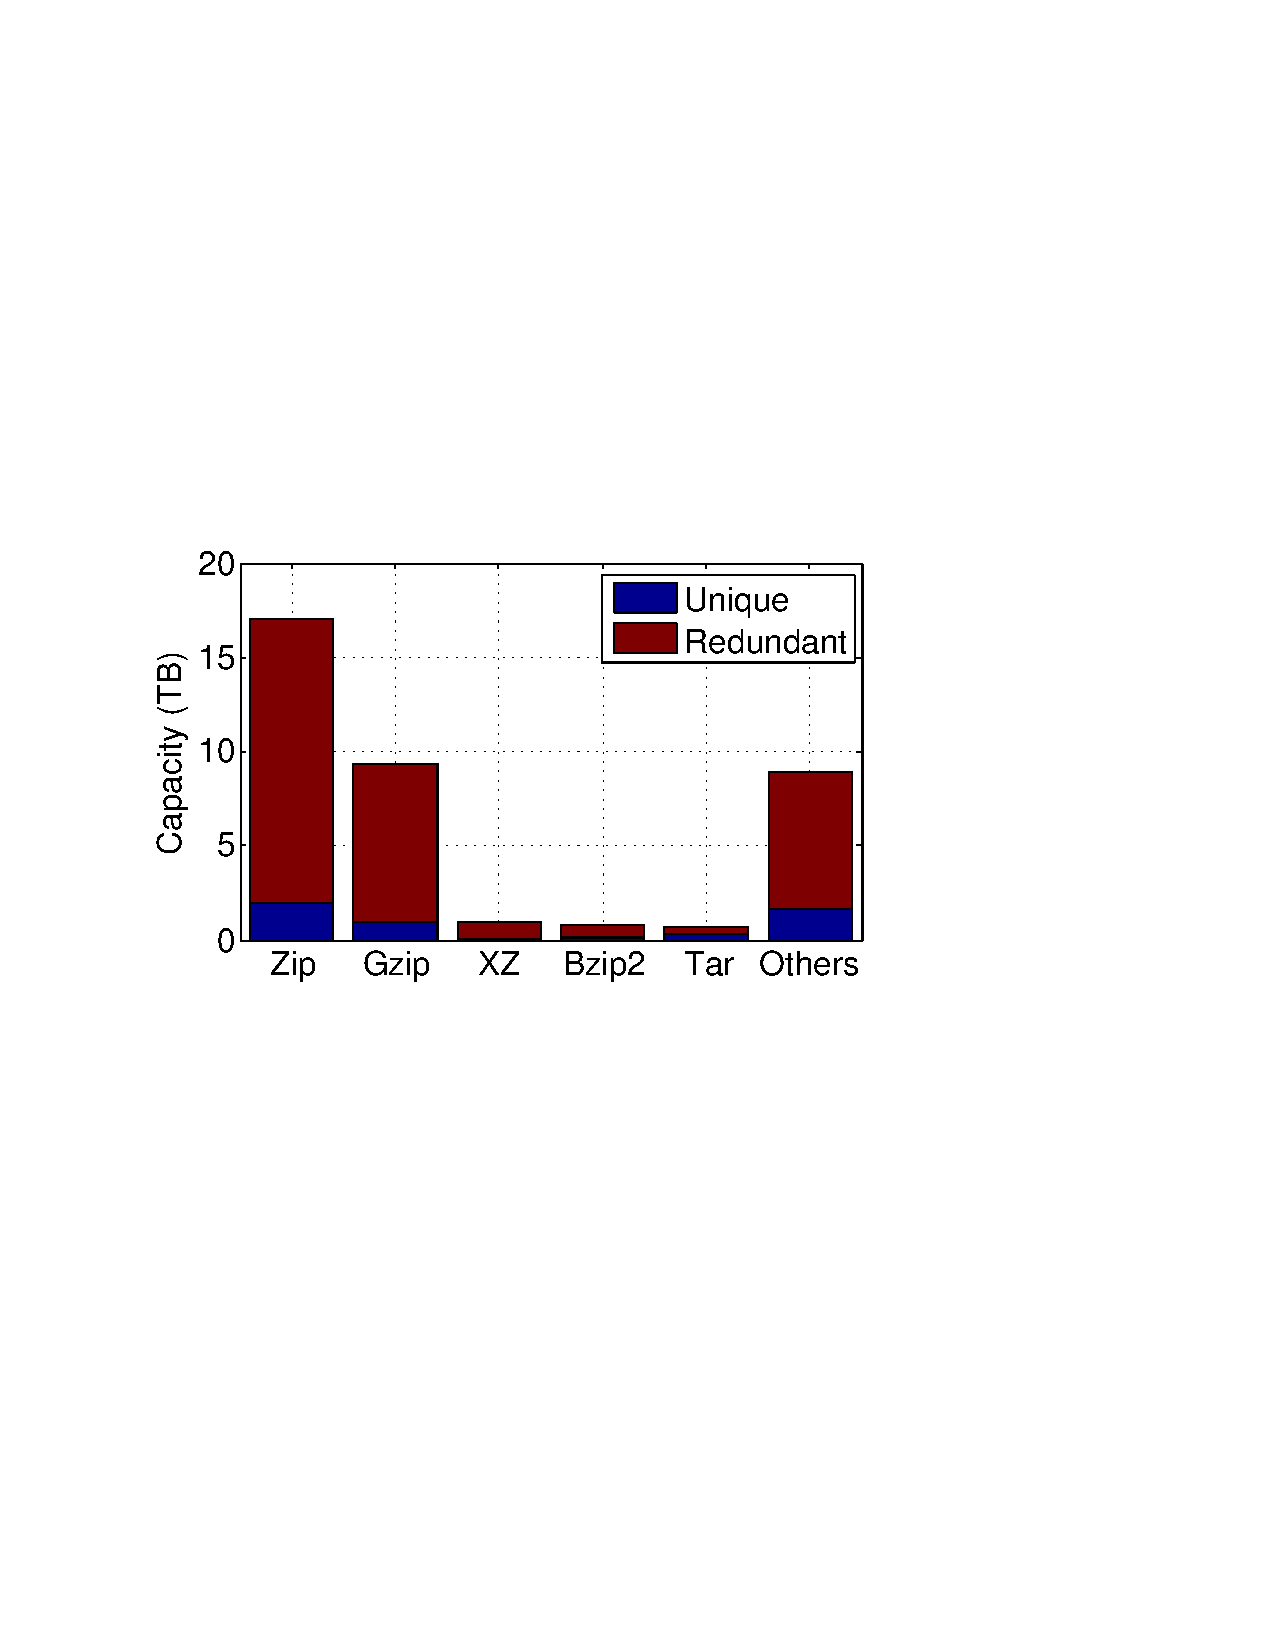
\includegraphics[width=0.45\textwidth]{graphs/type-tar-type}
	\caption{Tar file distribution.
	}
	\label{fig:file-type-tar}
\end{figure}

\subsection{Documents \& editors}

\begin{figure}
	\centering
	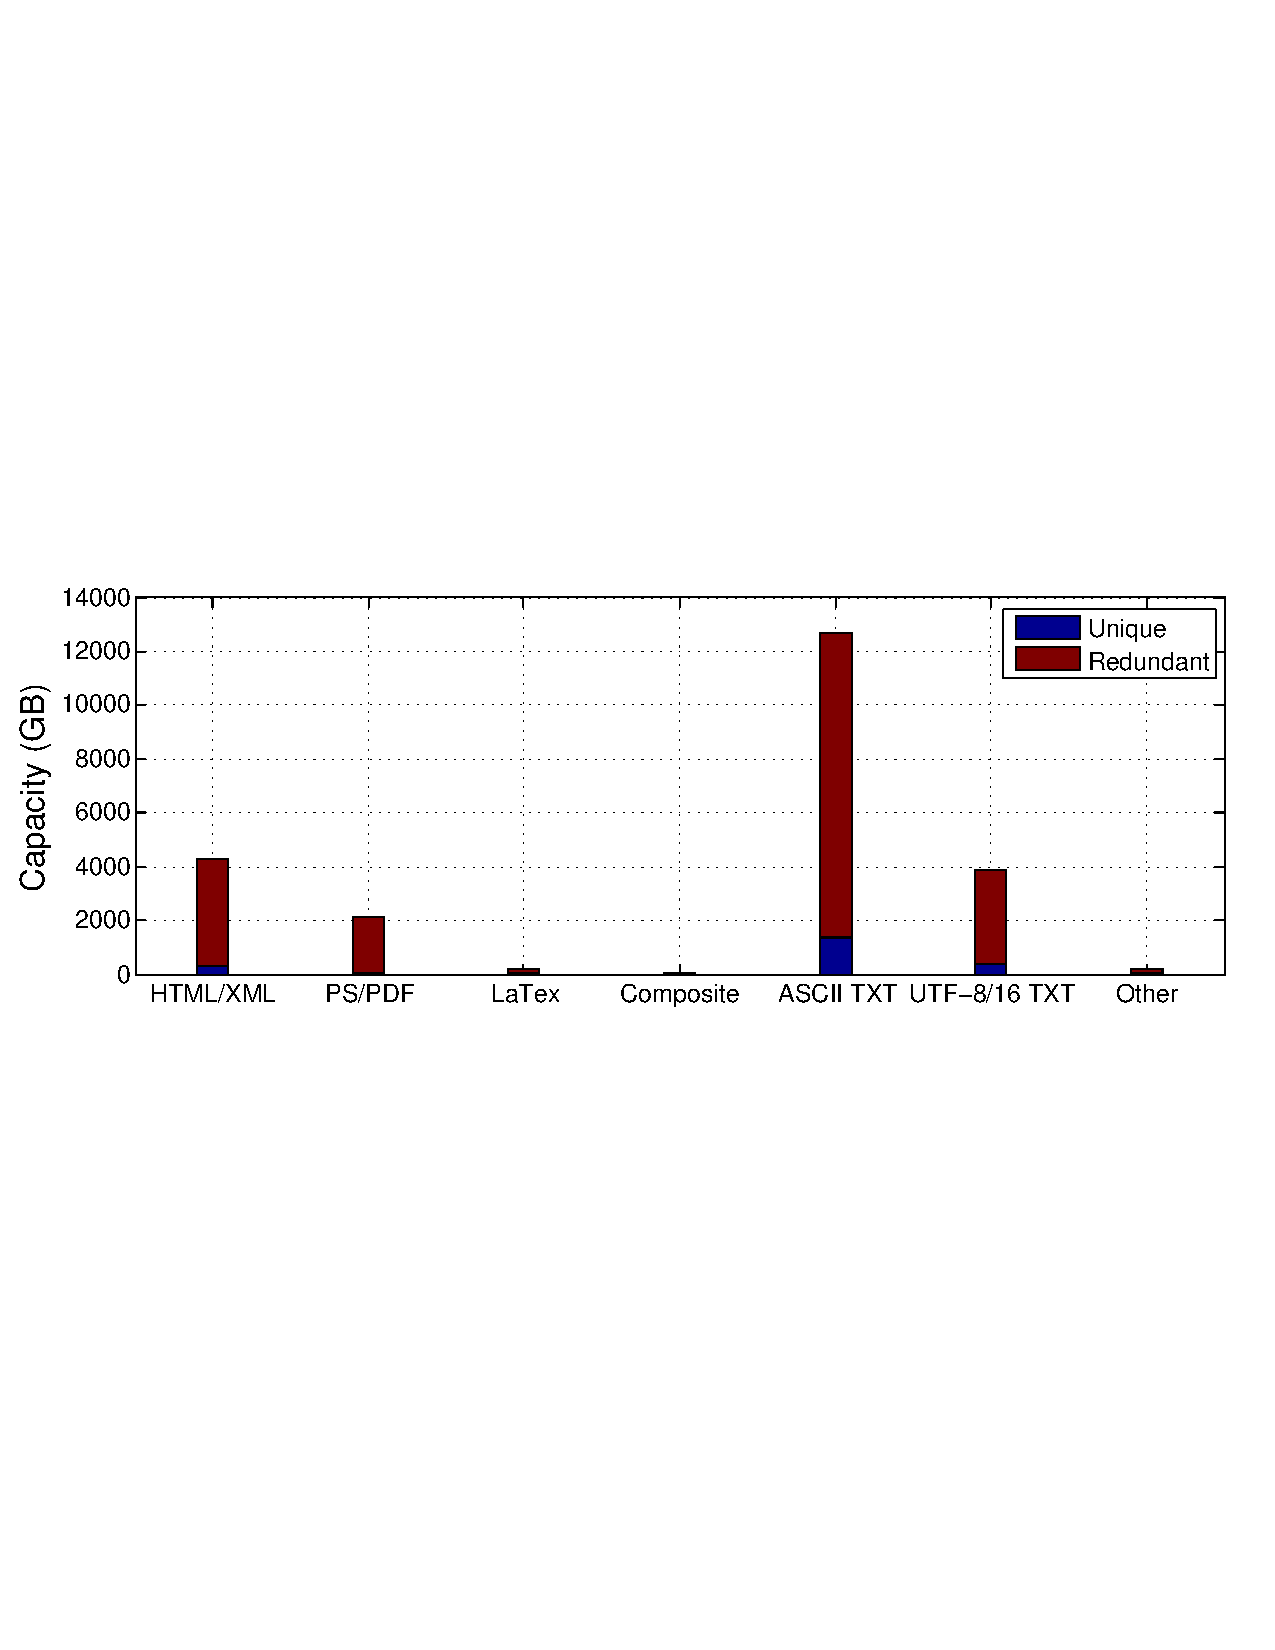
\includegraphics[width=0.5\textwidth]{graphs/type-utili-cap}
	\caption{Utility file distribution.
	}
	\label{fig:file_size}
\end{figure}

\subsection{Database}

\begin{figure*}[t]
	\centering
	\begin{minipage}{0.35\textwidth}
		\centering
		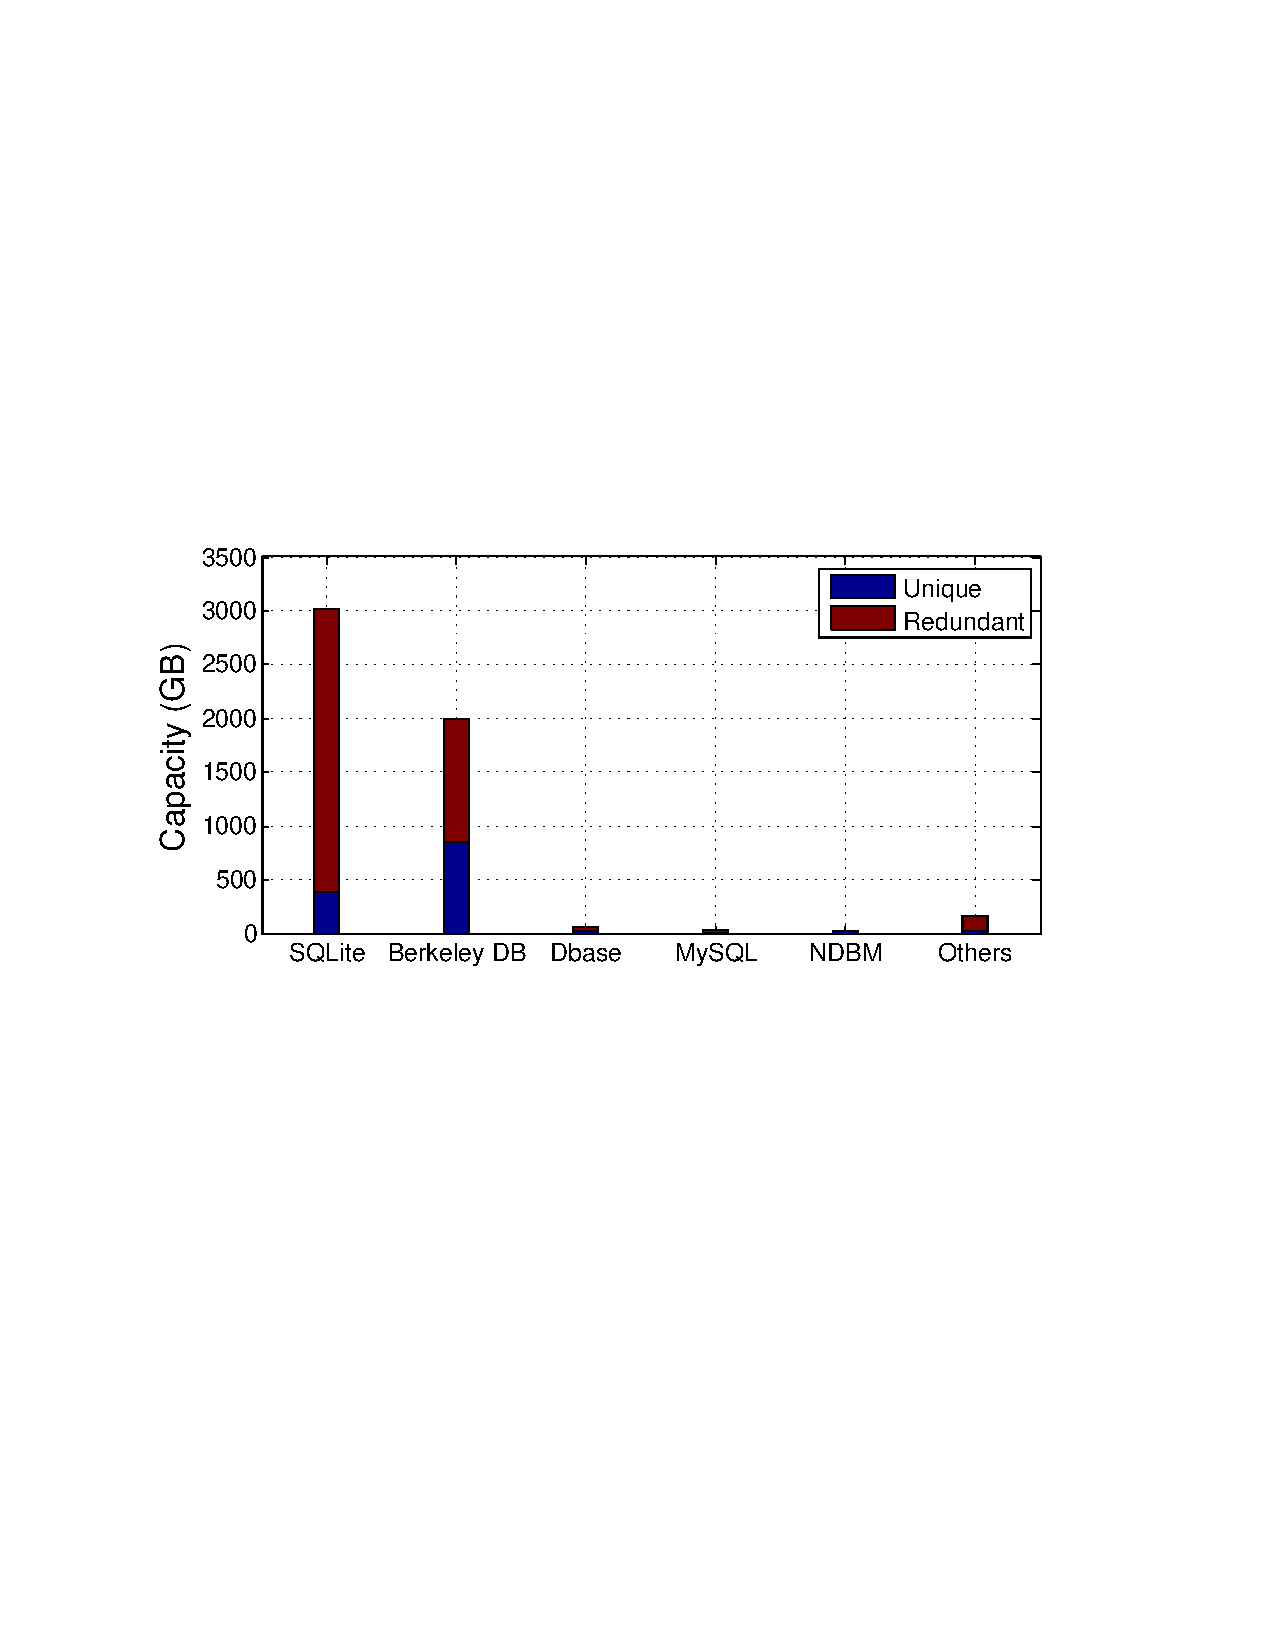
\includegraphics[width=1\textwidth]{graphs/type-db-cap.pdf}
		\caption{Database related files}
		\label{fig-dir}
	\end{minipage}%
	\begin{minipage}{0.3\textwidth}
		\centering
		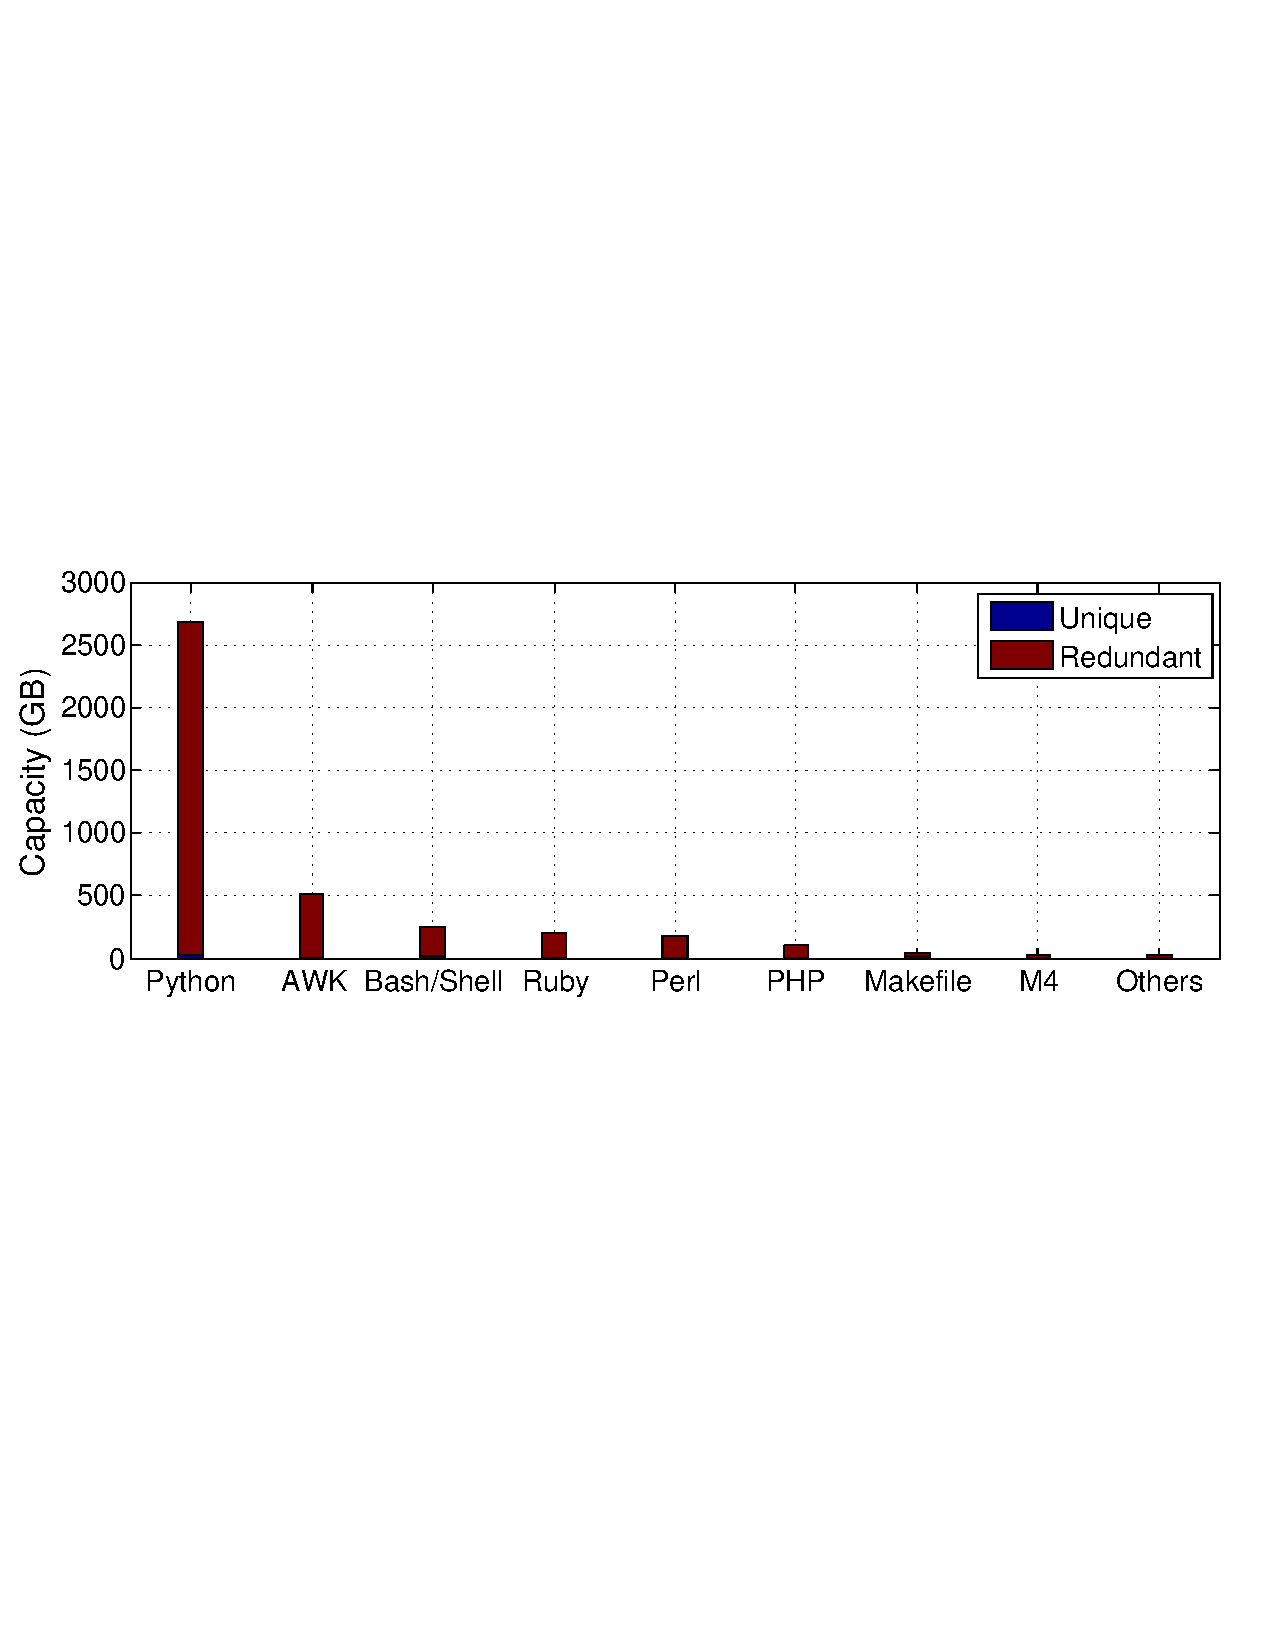
\includegraphics[width=1\textwidth]{graphs/type-script-cap}
		\caption{Script related files}
		\label{fig-file}
	\end{minipage}
	\begin{minipage}{0.3\textwidth}
		\centering
		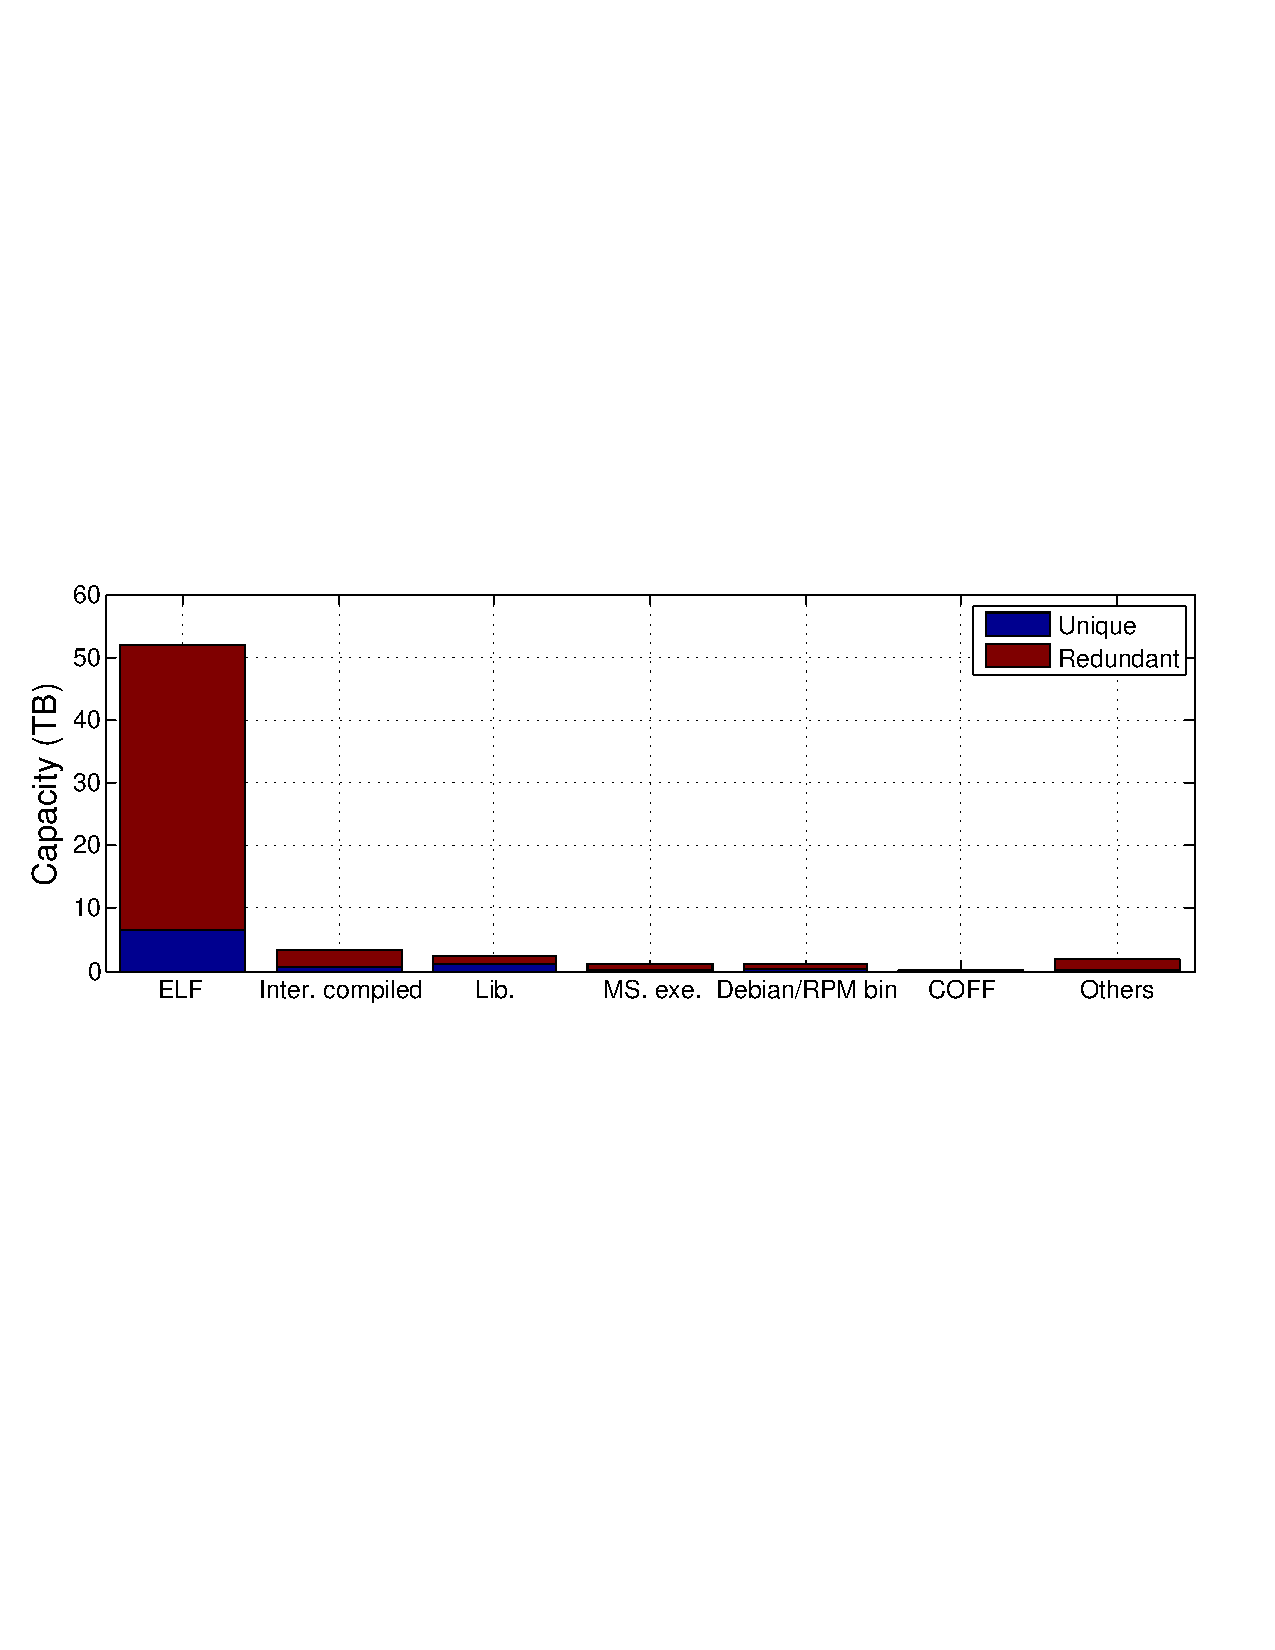
\includegraphics[width=1\textwidth]{graphs/type-exec-cap}
		\caption{Executables}
		\label{fig-file}
	\end{minipage}
\end{figure*}

\subsection{Images}

\begin{figure}
	\centering
	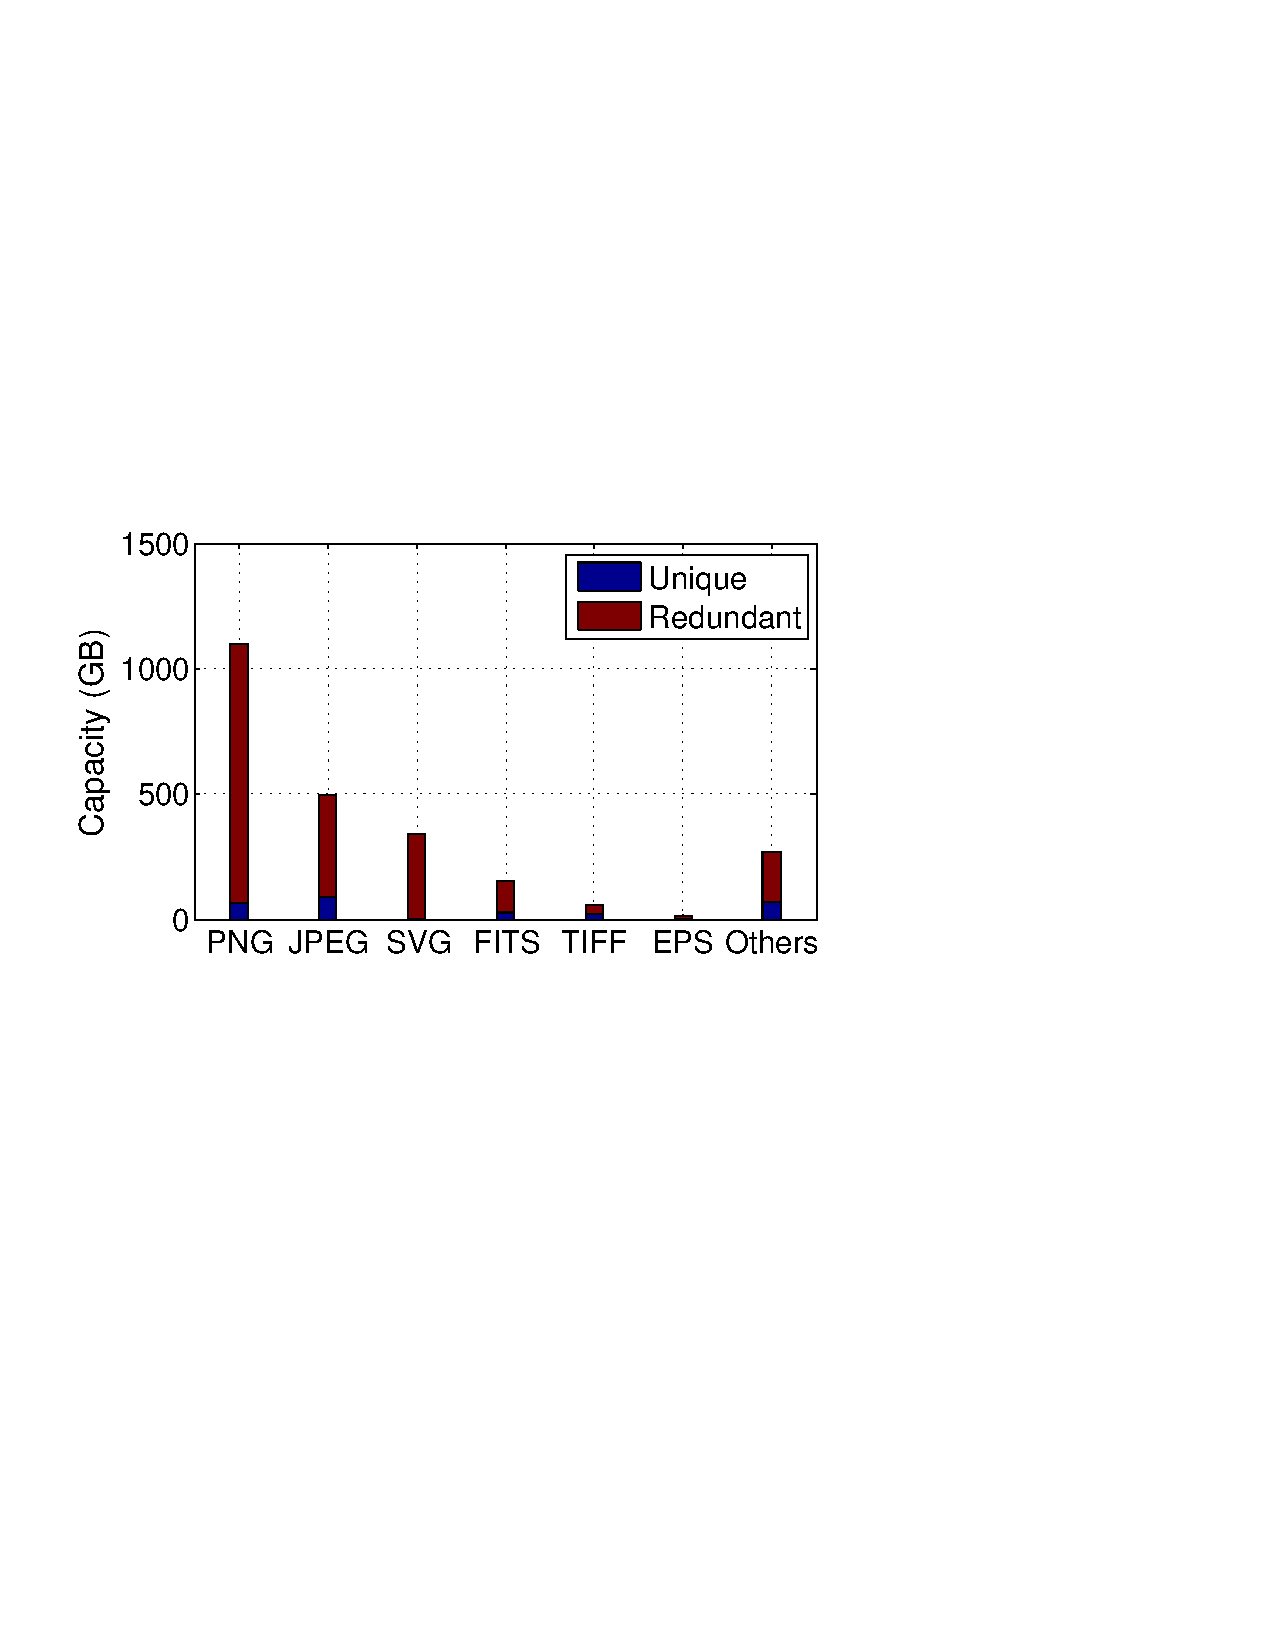
\includegraphics[width=0.35\textwidth]{graphs/type-image-cap}
	\caption{Utility file distribution.
	}
	\label{fig:file_size}
\end{figure}


%=======================================
%|             OLD VERSION              |
%=======================================

%\begin{table} 
%	\centering 
%	\scriptsize  
%	\caption{Top 20 redundant files' characterization (sorted by repeat cnt.)}
%	\label{tbl:top_dup_files_repeat_cnt} 
%	\begin{tabular}{|l|l|l|l|l|}%p{0.14\textwidth} 
%		\hline 
%		Filename & repeat cnt. & type & extension & size \\
%		\hline
%		&   &   &   &  \\
%		\hline
%		&   &   &   &   \\
%		\hline
%		&   &   &  &    \\
%		\hline
%		&  &  &  & \\
%		\hline
%		& &  &   & \\
%		\hline
%		& &  &   & \\
%		\hline
%		&  &  & & \\
%		\hline
%	\end{tabular} 
%\end{table}

%\begin{table} 
%	\centering 
%	\scriptsize  
%	\caption{Top 20 redundant files' characterization (sorted by capacity)} 
%	\label{tbl:top_dup_files_cap} 
%	\begin{tabular}{|l|l|l|l|l|}%p{0.14\textwidth} 
%		\hline 
%		Filename & repeat cnt. & type & extension & size \\
%		\hline
%		&   &   &   &  \\
%		\hline
%		&   &   &   &   \\
%		\hline
%		&   &   &  &    \\
%		\hline
%		&  &  &  & \\
%		\hline
%		& &  &   & \\
%		\hline
%		& &  &   & \\
%		\hline
%		&  &  & & \\
%		\hline
%	\end{tabular} 
%\end{table}


%\begin{table} 
%	\centering 
%	\scriptsize  
%	\caption{Top redundant file types} 
%	\label{tbl:top_dup_types} 
%	\begin{tabular}{|l|l|l|l|l|l|}%p{0.14\textwidth} 
%		\hline 
%		Type & extension & Num. & size & red. ratio (cnt.)  & red. ratio (cap.)\\
%		\hline
%		&   &   &  & &   \\
%		\hline
%		&   &   &  & &    \\
%		\hline
%		&   &   &   & &   \\
%		\hline
%		&  &  &  & & \\
%		\hline
%		& &  &  & & \\
%		\hline
%		& &  & & &  \\
%		\hline
%		&  &  & & &  \\
%		\hline
%	\end{tabular} 
%\end{table} 

%\subsection{Redundant ratio for directories}
%
%\begin{table} 
%	\centering 
%	\scriptsize  
%	%\begin{minipage}{.5\linewidth}
%	\caption{Inter-dir redundant ratio for dirs in terms of file count and capacity} \label{tbl:intra_dup_ratio_dirs} 
%	\begin{tabular}{|l|l|l|}%p{0.14\textwidth} 
%		\hline 
%		% after \\: \hline or \cline{col1-col2} \cline{col3-col4} ... 
%		% after \\: \hline or \cline{col1-col2} \cline{col3-col4} ... 
%		& File count & Capacity \\
%		\hline
%		Avg. & 98.75\% & 97.33\%\\
%		\hline
%		Median & - & - \\
%		\hline
%		Max. & 1 & 1\\
%		\hline
%		Min.  & 0.87\%  & $<$ 0.00\%\\
%		\hline
%		Stdev.  &  4.70\% & 10.49\\
%		\hline
%		Layer dataset after share.-dedup (Uncompressed) & -  & -\\
%		\hline 
%		Total layer dataset (Uncompressed) &  -	& -\\
%		\hline
%	\end{tabular} 
%\end{table}
%
%\begin{table} 
%	\centering 
%	\scriptsize  
%	%\begin{minipage}{.5\linewidth}
%	\caption{Intra-dir redundant ratio for dirs in terms of file count and capacity} \label{tbl:inter_dup_ratio_dirs} 
%	\begin{tabular}{|l|l|l|}%p{0.14\textwidth} 
%		\hline 
%		% after \\: \hline or \cline{col1-col2} \cline{col3-col4} ... 
%		% after \\: \hline or \cline{col1-col2} \cline{col3-col4} ... 
%		& File count & Capacity \\
%		\hline
%		Avg. & 98.75\% & 97.33\%\\
%		\hline
%		Median & - & - \\
%		\hline
%		Max. & 1 & 1\\
%		\hline
%		Min.  & 0.87\%  & $<$ 0.00\%\\
%		\hline
%		Stdev.  &  4.70\% & 10.49\\
%		\hline
%		Layer dataset after share.-dedup (Uncompressed) & -  & -\\
%		\hline 
%		Total layer dataset (Uncompressed) &  -	& -\\
%		\hline
%	\end{tabular} 
%\end{table}

%\subsection{Redundant directory characterization}
%
%\begin{table} 
%	\centering 
%	\scriptsize  
%	%\begin{minipage}{.5\linewidth}
%	\caption{Top redundant dirs'characterization} 
%	\label{tbl:top_dup_dirs} 
%	\begin{tabular}{|l|l|l|l|}%p{0.14\textwidth} 
%		\hline 
%		% after \\: \hline or \cline{col1-col2} \cline{col3-col4} ... 
%		% after \\: \hline or \cline{col1-col2} \cline{col3-col4} ... 
%		Name & Num. & Redundant ratio & Avg. size \\
%		\hline
%		home &   &   &     \\
%		\hline
%		&   &   &      \\
%		\hline
%		&   &   &      \\
%		\hline
%		&  &  &  \\
%		\hline
%		& &  &   \\
%		\hline
%		& &  &   \\
%		\hline
%		&  &  & \\
%		\hline
%	\end{tabular} 
%\end{table} 

%\begin{figure}
%	\centering
%	\includegraphics[width=0.5\textwidth]{graphs/}
%	\caption{CDF of file repeat count.
%	}
%	\label{fig:file_repeat_count}
%\end{figure}

%\paragraph{Cumulative distribution and probability distribution of file size in terms of unique file size, redundant file size, overall file size}


%\paragraph{Average file size by repeat count}
%
%There is no relation between file repeat count and average file size.
%
%\begin{figure}
%	\centering
%	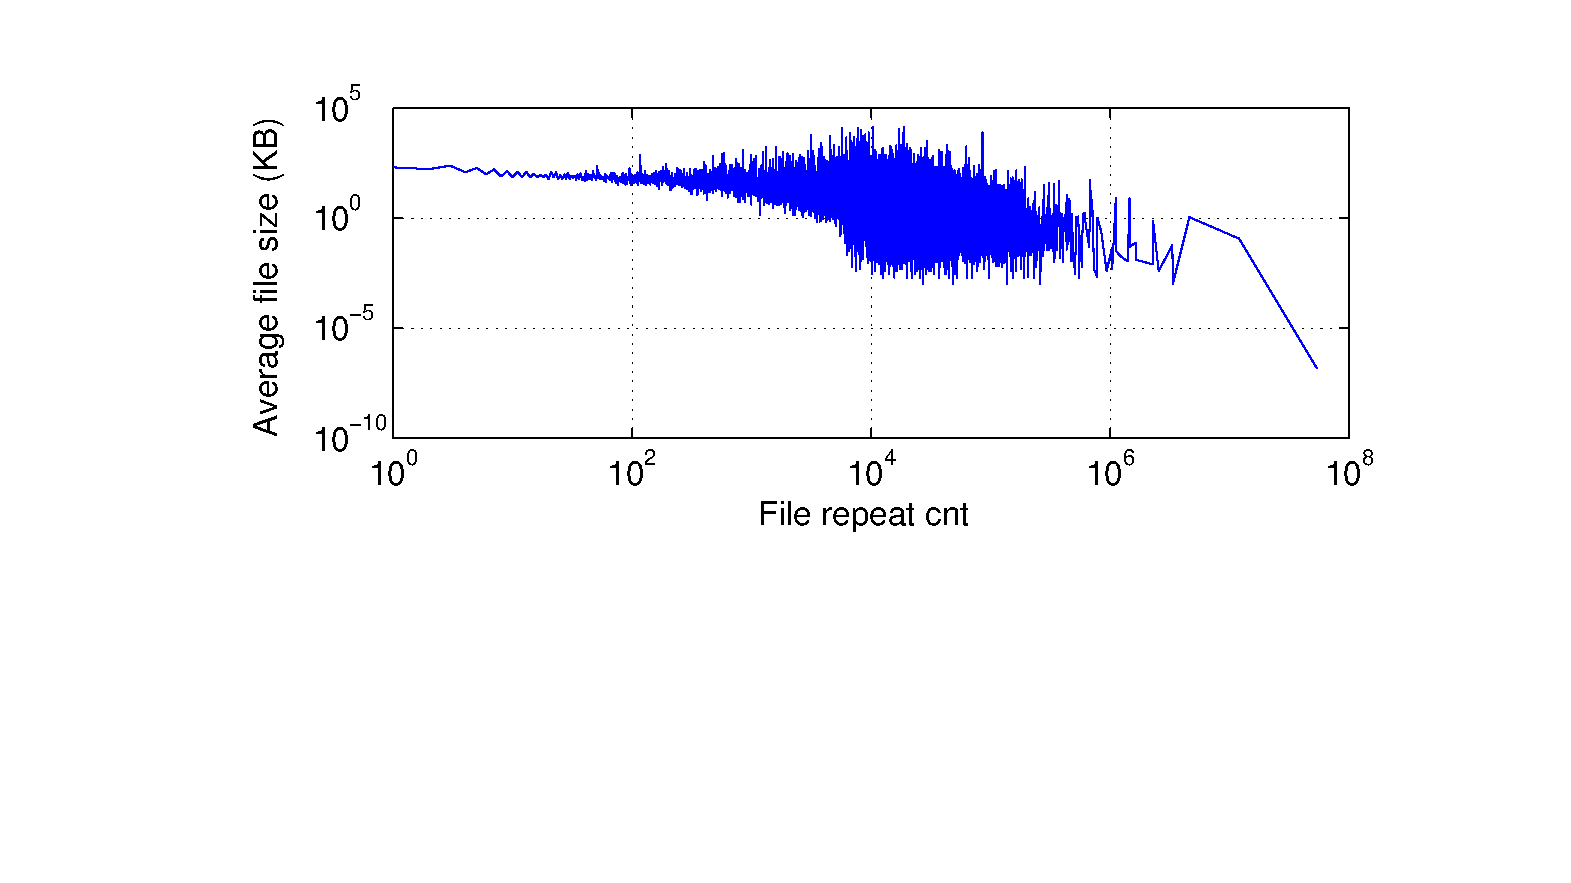
\includegraphics[width=0.5\textwidth]{graphs/avg_size_by_cnt.eps}
%	\caption{Average file size with same repeat count.
%	}
%	\label{fig_avg_size_by_cnt}
%\end{figure}
%
%\paragraph{Redundant ratio by file size for the files with the same content in terms of file count and storage capacity}
%Total size of redundant files with same content(TRS)
%
%97\% of the TRSs are equal or less than 100MB.
%
%\begin{figure}
%	\centering
%	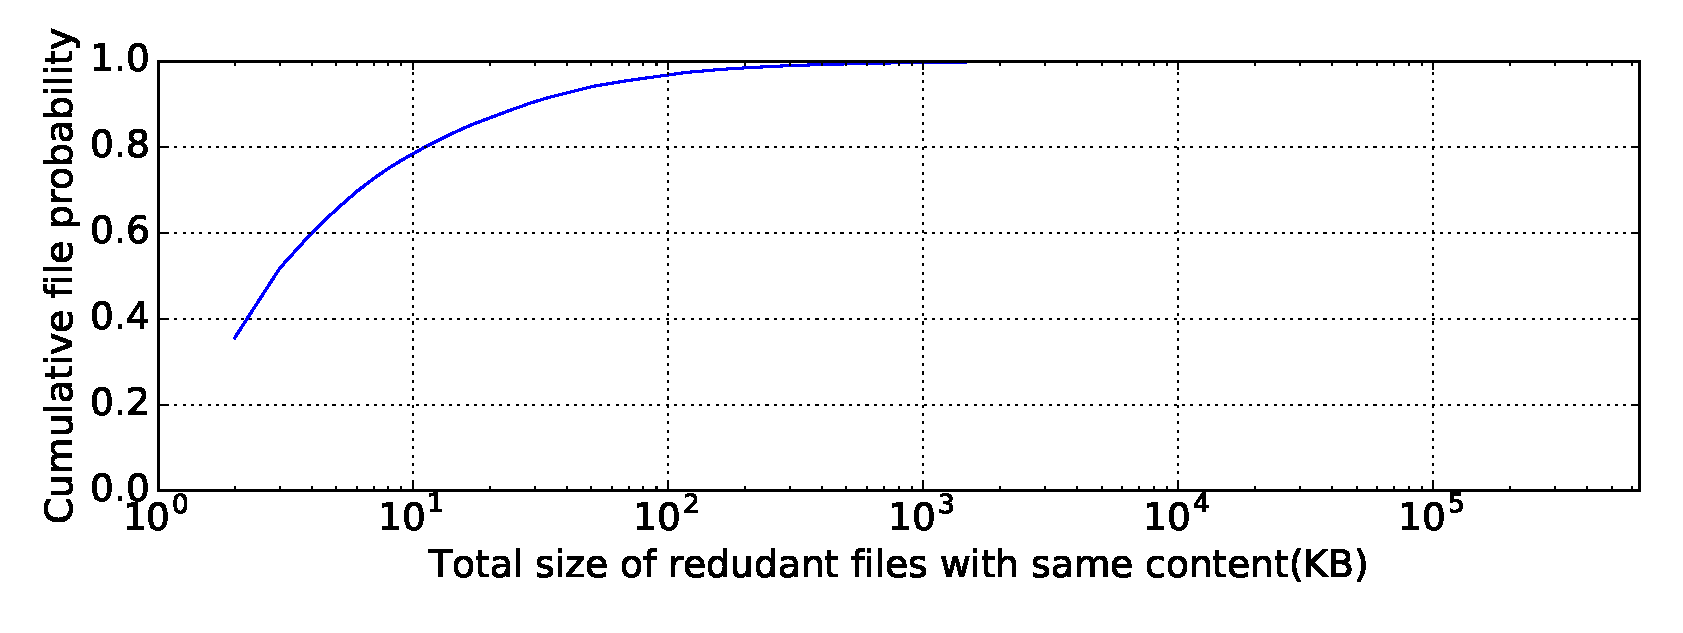
\includegraphics[width=0.5\textwidth]{graphs/Total_size_of_redudant_files_with_same_content-KB.eps}
%	\caption{CDF of total file size with same file content (MB).
%	}
%	\label{fig_total_redundant_same_digest}
%\end{figure}
%
%\paragraph{Redundant ratio by repeat count for the files with the same repeat count in terms of file count and storage capacity}
%
%However, with the increase of file repeat count, the sum of file size with same repeat count becomes smaller.
%
%\begin{figure}
%	\centering
%	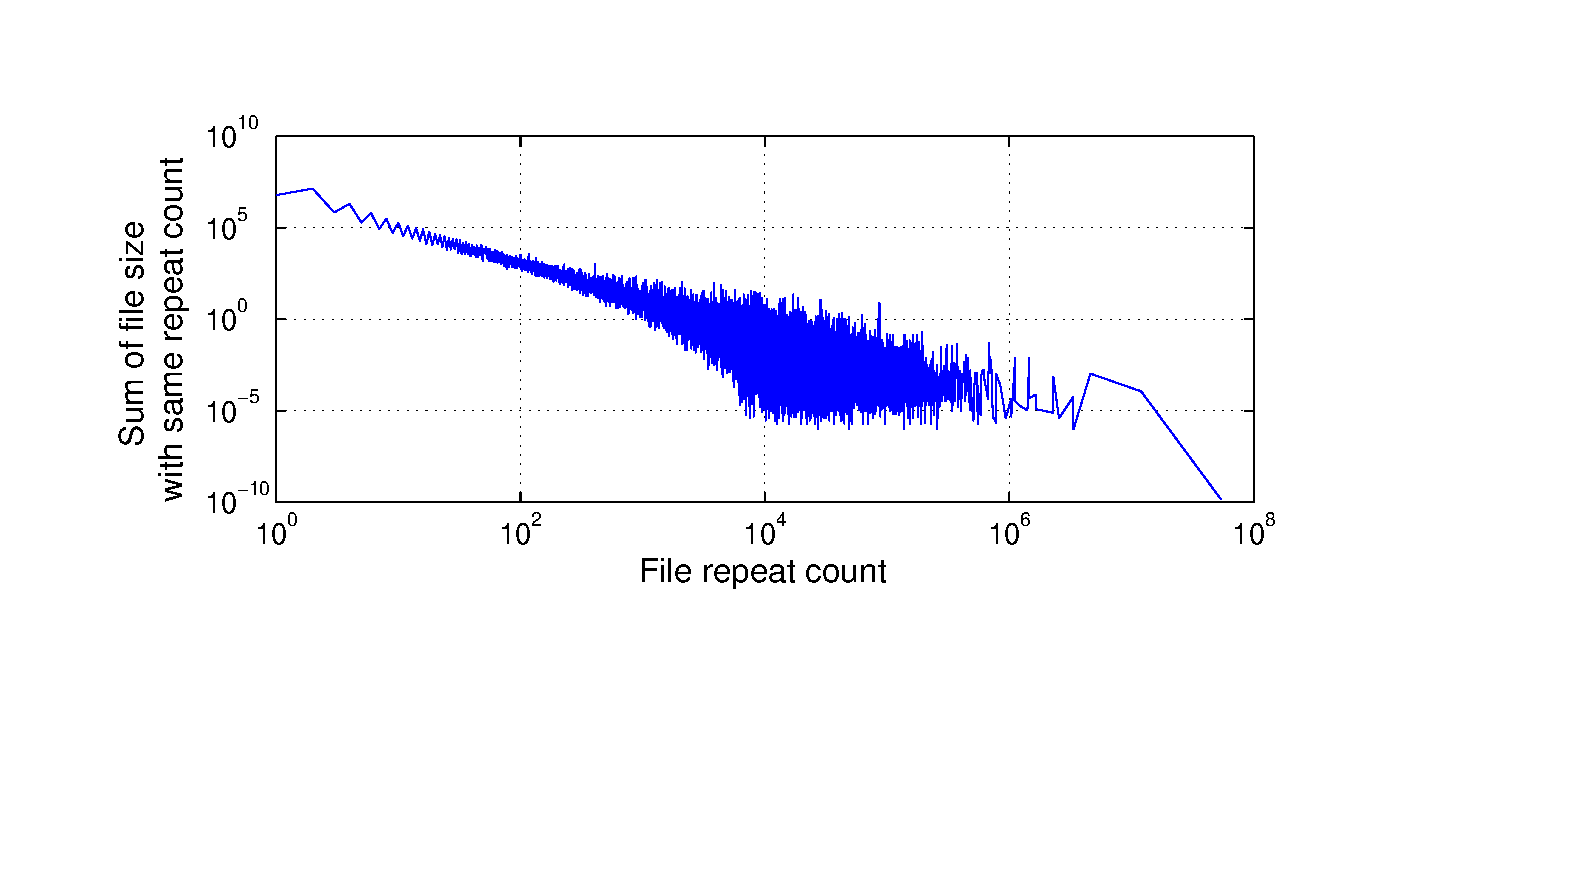
\includegraphics[width=0.5\textwidth]{graphs/sum_size_by_cnt.eps}
%	\caption{Sum of file size with same repeat count.
%	}
%	\label{fig_sum_by_cnt}
%\end{figure}

%
%\paragraph{Cumulative distribution and probability distribution of file repeat count}
%\begin{table} 
%	\centering 
%	\scriptsize  
%	%\begin{minipage}{.5\linewidth}
%	\caption{Summary of image types} \label{tbl:redundant_ratio} 
%	\begin{tabular}{|l|l|l|}%p{0.14\textwidth} 
%		\hline 
%		% after \\: \hline or \cline{col1-col2} \cline{col3-col4} ... 
%		% after \\: \hline or \cline{col1-col2} \cline{col3-col4} ... 
%		Image types & num. & avg. redundant ratio  \\
%		\hline
%		  &   &        \\
%		\hline
%		  &   &         \\
%		\hline
%		   &   &       \\
%		   \hline
%		other     &   &       \\
%		\hline
%	\end{tabular} 
%\end{table}

%\subsection{Redundant files with same filename and relative path}
%
%\subsection{Common directories that contains redundant files}
%
%\subsection{Redundant tar files}
%\begin{table} 
%	\centering 
%	\scriptsize  
%	%\begin{minipage}{.5\linewidth}
%	\caption{Summary of file \& dir. characterization} \label{tbl:sum_file_dir_char} 
%	\begin{tabular}{|l|l|l|l|l|}%p{0.14\textwidth} 
%		\hline 
%		% after \\: \hline or \cline{col1-col2} \cline{col3-col4} ... 
%		% after \\: \hline or \cline{col1-col2} \cline{col3-col4} ... 
%		Metrics & max & min & median & avg.\\
%		\hline
%		File size &   &   &   &  \\
%		\hline
%		File size (repeat cnt. $>$ 1) &   &   &    &  \\
%		\hline
%		File size (repeat cnt. $=$ 1) &   &   &    &  \\
%		\hline
%		\hline
%		Dir. size &  &  & & \\
%		\hline
%		File cnt. per dir & &  &  & \\
%		\hline
%		Redundant ratio & &  &  & \\
%		\hline
%		Dir. depth  &  &  & & \\
%		\hline
%	\end{tabular} 
%\end{table} 